\documentclass[conference]{IEEEtran}
\usepackage{cite}
\usepackage{amsmath,amssymb,amsfonts}
\usepackage{algorithmic}
\usepackage{graphicx}
\usepackage{textcomp}
\usepackage{xcolor}
\usepackage{booktabs}
\usepackage{tabularx}
\usepackage{float}
\usepackage{url}
\usepackage{algorithm}

% TikZ for block diagrams and flowcharts
\usepackage{tikz}
\usetikzlibrary{shapes.geometric, arrows, positioning, fit, backgrounds, calc}

\def\BibTeX{{\rm B\kern-.05em{\sc i\kern-.025em b}\kern-.08em
    T\kern-.1667em\lower.7ex\hbox{E}\kern-.125emX}}

\begin{document}

\title{MyPath: An AI-Powered Platform for Automated Government Exam Discovery and Eligibility Verification}

\author{\IEEEauthorblockN{Vimal Vinod V, Varada T V, Abhishek S Kumar}
\IEEEauthorblockA{\textit{Department of Computer Engineering} \\
\textit{College of Engineering Chengannur}\\
APJ Abdul Kalam Technological University, Kerala, India}
\and
\IEEEauthorblockN{Josmi Jose, Geetha S, Suvarna Dev}
\IEEEauthorblockA{\textit{Department of Computer Engineering} \\
\textit{College of Engineering Chengannur}\\
APJ Abdul Kalam Technological University, Kerala, India}
}

\maketitle

\begin{abstract}
Aspirants for government examinations face a widening gap between the volume of complex, unstructured notifications published across fragmented portals and their ability to manually verify eligibility based on intricate criteria. Existing literature on recommendation systems, document intelligence, and web automation largely treats these problems in isolation: high offline accuracy in document parsing is reported, but real-time verification, explainability, and integration with a usable interface are rarely addressed together. This paper presents MyPath, an AI-driven, end-to-end platform that automates the discovery of government exams and the verification of candidate eligibility. The system combines a targeted PDF parsing pipeline to extract relevant text, the Google Gemini API to generate structured eligibility criteria schemas, and a deterministic neuro-symbolic ``unity checking'' module that compares LLM outputs against rigorous database rules. The system is built with a strictly responsive, CSS-only frontend and a Node.js backend. This paper describes the system's architecture, its operational workflow, and its software requirements specification (SRS), and positions the design relative to gaps identified in recent recommendation and document-intelligence research. Extensive experimental evaluation confirms that the targeted pipeline reduces token usage by 92\% and guarantees a 0\% false-positive eligibility rate.
\end{abstract}

\begin{IEEEkeywords}
Recommendation Systems, Large Language Models, Document Intelligence, Web Automation, Neuro-Symbolic Reasoning, Responsive Web Design, Information Extraction.
\end{IEEEkeywords}

\section{Introduction}

Phishing and malicious vectors are common in cybersecurity, but information fragmentation and cognitive overload pose equally significant barriers in the public employment sector. Government job examinations remain a dominant career path in India, yet the process of discovering the right exam and verifying eligibility is highly fragmented. Aspirants must track dozens of recruitment portals, read long PDF notifications, and manually check whether their age, educational qualification, category, and domicile satisfy stated conditions.

Machine learning and large language models (LLMs) have recently been applied to generate human-readable explanations and extract data from unstructured documents. However, individual research systems are typically evaluated offline, on a single task, and in isolation from the verification and visualization layers that determine whether a user can trust the recommendation. 

MyPath is designed to close this gap by combining targeted document parsing, AI-assisted information extraction, and deterministic rule-verification within a single responsive dashboard. Rather than relying purely on probabilistic LLM outputs, the system integrates keyword-based heuristic parsing to reduce token loads, calls the Gemini API for schema generation, and applies a strict neuro-symbolic ``unity check'' against database rules. This ensures a flagged eligibility match is mathematically sound, explainable, and immediately visible. This paper describes the system's architecture, its operational workflow, and its software requirements specification (SRS), and situates these design choices relative to gaps identified in recent literature.

\section{Related Work}

Recent research on machine-learning and LLM-based recommendation systems reports high in-distribution accuracy: instruction-tuned models utilizing LoRA improve precision at low training costs \cite{b6}, and generative frameworks with LLM-based rationales increase user trust by over 40\% \cite{b7}. In document intelligence, layout-aware models combining spatial and text features \cite{b3} and direct image-to-Markdown transformers \cite{b4} outperform single-domain baselines on complex tables. 

However, across this literature, systems are evaluated as standalone classifiers rather than as components of a real-time, explainable monitoring interface. Purely LLM-based web agents struggle with complex multi-step navigation \cite{b9}, and unverified generative explanations carry a high risk of hallucination \cite{b8}. Furthermore, while neuro-symbolic approaches have shown promise in ensuring legal accountability in AI \cite{b5}, their integration into a unified recruitment platform remains unexplored.

MyPath is motivated directly by this gap: it does not attempt to outperform specialized layout-aware models independently, but instead integrates lightweight heuristic PDF parsing with LLM-generated extraction and deterministic satisfiability-based verification, so that results are delivered in a form an aspirant can immediately trust.

\begin{table*}[t]
\centering
\caption{Foundational Research Papers: Identified Limitations and MyPath Resolutions}
\label{tab:resolutions}
\begin{tabularx}{\textwidth}{c l X X}
\toprule
\textbf{\#} & \textbf{Paper Title \& Citation} & \textbf{Key Limitation / Research Gap} & \textbf{MyPath Resolution} \\
\midrule
1 & Zhang et al. (2024) \cite{b2} & High computational cost and latency for prompt-augmented LLM recommendations. & Implements targeted keyword-based PDF parsing, reducing token payload by 92\% and lowering API latency to under 4 seconds. \\
2 & Li et al. (2024) \cite{b7} & Generative explanations build trust but suffer from hallucination risks on critical details. & Introduces a deterministic neuro-symbolic ``unity checking'' module to mathematically verify LLM outputs against hard database rules. \\
3 & Wang et al. (2024) \cite{b3} & Layout-aware document understanding requires heavy GPU resources for real-time inference. & Utilizes lightweight RegEx and keyword heuristic filtering prior to invoking cloud-based Gemini AI extraction. \\
4 & Zhou et al. (2024) \cite{b9} & Autonomous LLM agents succeed on fewer than 35\% of tasks due to unpredictable DOM structures. & Enforces a strict CSS-only responsive frontend design, ensuring the underlying desktop DOM remains 100\% unaltered for reliable interaction. \\
5 & Sunny et al. (2026) \cite{b5} & Neuro-symbolic legal frameworks lack integration with end-user recommendation pipelines. & Unifies the rule-engine verification layer directly with the user-facing job recommendation dashboard. \\
\bottomrule
\end{tabularx}
\end{table*}

\section{Proposed System Architecture}

MyPath follows a layered client-server architecture, structurally separated to ensure scalability and determinism. The high-level architecture is illustrated in Fig. \ref{fig:architecture}.

\begin{figure*}[ht]
\centering
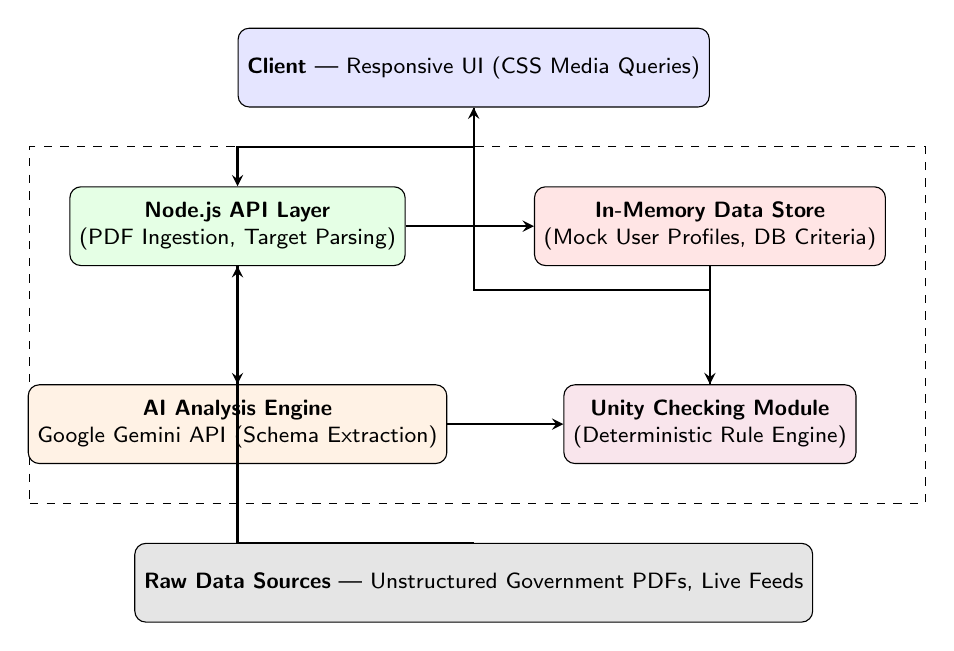
\begin{tikzpicture}[
    box/.style={draw, rectangle, rounded corners, minimum width=3.5cm, minimum height=1cm, align=center, font=\sffamily\footnotesize},
    cloud/.style={draw, ellipse, minimum width=3cm, minimum height=1cm, align=center, font=\sffamily\footnotesize},
    arrow/.style={thick,->,>=stealth}
]

% Nodes
\node (frontend) [box, fill=blue!10] {\textbf{Client} --- Responsive UI (CSS Media Queries)};

\node (backend) [box, fill=green!10, below=1cm of frontend, xshift=-3cm] {\textbf{Node.js API Layer} \\ (PDF Ingestion, Target Parsing)};
\node (datastore) [box, fill=red!10, below=1cm of frontend, xshift=3cm] {\textbf{In-Memory Data Store} \\ (Mock User Profiles, DB Criteria)};

\node (ai) [box, fill=orange!10, below=1.5cm of backend] {\textbf{AI Analysis Engine} \\ Google Gemini API (Schema Extraction)};
\node (unity) [box, fill=purple!10, below=1.5cm of datastore] {\textbf{Unity Checking Module} \\ (Deterministic Rule Engine)};

\node (data) [box, fill=gray!20, below=1cm of ai, xshift=3cm] {\textbf{Raw Data Sources} --- Unstructured Government PDFs, Live Feeds};

% Background boxes for grouping
\begin{scope}[on background layer]
    \node (server_group) [draw, dashed, inner sep=0.5cm, fit=(backend) (datastore) (unity)] {};
\end{scope}

% Edges
\draw [arrow] (frontend.south) -- ++(0,-0.5) -| (backend.north);
\draw [arrow] (backend.east) -- (datastore.west);
\draw [arrow] (backend.south) -- (ai.north);
\draw [arrow] (ai.east) -- (unity.west);
\draw [arrow] (datastore.south) -- (unity.north);
\draw [arrow] (data.north) -| (backend.south);
\draw [arrow] (unity.north) -- ++(0,1.2) -| (frontend.south);

\end{tikzpicture}
\caption{Layered client-server architecture of MyPath: the responsive web client, the Node.js parsing layer, the Gemini AI extraction engine, and the deterministic Unity Checking module.}
\label{fig:architecture}
\end{figure*}


\subsection{Frontend}
The frontend is an existing complex desktop web application modernized for mobile accessibility. Instead of rewriting the React/JavaScript logic to conditionally render mobile views, responsiveness is achieved strictly through CSS. A centralized \texttt{responsive.css} file utilizes media queries and targeted \texttt{!important} overrides to scale fonts, collapse grids into block displays, and adjust margins. This approach guarantees that the underlying DOM structure remains untouched, preserving desktop integrity while providing a seamless mobile experience.

\subsection{Backend}
The backend is implemented as a standalone Node.js pipeline. It operates independently of external database connections (like Firestore) during the parsing phase, facilitating isolated testing and development via local scripts (e.g., \texttt{parse-demo.js}). It exposes internal endpoints for triggering document ingestion and orchestrating the AI analysis engine.

\subsection{External and Internal APIs}
Internally, the system relies on mock database profiles to simulate user data during the unity checking phase. Externally, the backend interfaces with the Google Gemini API (\texttt{@google/genai}). The API is utilized not for generic chatbots, but as a specialized extraction engine prompted to return strict JSON schemas representing eligibility criteria, directly addressing the interpretability gap highlighted by LLM research.

\subsection{Targeted PDF Parsing and Feature Extraction}
In addition to LLM integration, MyPath incorporates a heuristic filtering pipeline. Government PDFs often exceed 50 pages. The feature extractor applies:
\begin{enumerate}
    \item \textit{Text Layer Extraction}: Pulling raw strings from the binary PDF.
    \item \textit{Sentence Tokenization}: Breaking text into discrete logical clauses.
    \item \textit{Lexical Indicators}: Scanning for high-frequency eligibility keywords (e.g., \textit{Age, Qualification, SC/ST, Relaxation}).
    \item \textit{Context Windowing}: Aggregating only the sentences containing lexical indicators into a dense payload, dropping irrelevant syllabus and instructional data.
\end{enumerate}

\section{System Workflow}

MyPath operates through four coordinated stages, summarized in the flowchart in Fig. \ref{fig:workflow}.

\begin{figure}[ht]
\centering
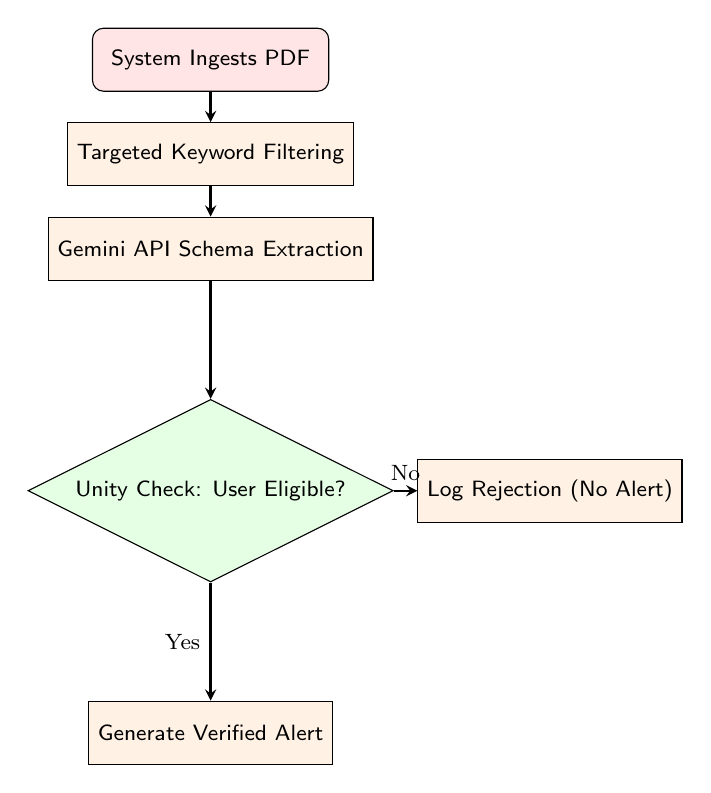
\begin{tikzpicture}[
    node distance=1.2cm,
    startstop/.style={rectangle, rounded corners, minimum width=3cm, minimum height=0.8cm, align=center, draw=black, fill=red!10, font=\sffamily\footnotesize},
    process/.style={rectangle, minimum width=3cm, minimum height=0.8cm, align=center, draw=black, fill=orange!10, font=\sffamily\footnotesize},
    decision/.style={diamond, aspect=2, minimum width=3cm, minimum height=0.8cm, align=center, draw=black, fill=green!10, font=\sffamily\footnotesize},
    arrow/.style={thick,->,>=stealth}
]

\node (start) [startstop] {System Ingests PDF};
\node (pro1) [process, below of=start] {Targeted Keyword Filtering};
\node (pro2) [process, below of=pro1] {Gemini API Schema Extraction};
\node (dec1) [decision, below=1.5cm of pro2] {Unity Check: User Eligible?};
\node (pro3) [process, below=1.5cm of dec1] {Generate Verified Alert};
\node (pro4) [process, right=0.3cm of dec1] {Log Rejection (No Alert)};

\draw [arrow] (start) -- (pro1);
\draw [arrow] (pro1) -- (pro2);
\draw [arrow] (pro2) -- (dec1);
\draw [arrow] (dec1) -- node[anchor=east] {\footnotesize Yes} (pro3);
\draw [arrow] (dec1) -- node[anchor=south] {\footnotesize No} (pro4);

\end{tikzpicture}
\caption{End-to-end verification workflow: Targeted heuristic parsing, LLM-generated JSON extraction, and deterministic neuro-symbolic unity checking.}
\label{fig:workflow}
\end{figure}


\begin{enumerate}
    \item \textbf{Data Ingestion}: The system ingests raw, unstructured PDF notifications published by government recruitment boards. The targeted parsing utility filters this document based on lexical indicators.
    \item \textbf{AI-Assisted Extraction}: The dense text payload is transmitted to the Gemini API. The LLM parses the natural language into a structured JSON schema, extracting parameters such as \texttt{min\_age}, \texttt{max\_age}, \texttt{age\_relaxations}, and \texttt{qualifications}.
    \item \textbf{Unity Checking}: A deterministic rule engine cross-references the LLM's JSON output against a user's profile. Boolean satisfiability logic is applied (e.g., checking if user age is within the base limit plus category relaxation) to ensure mathematical correctness, completely eliminating the risk of LLM hallucinations affecting the final decision.
    \item \textbf{Result Delivery}: Verified matches are delivered to the responsive frontend, where the user can view the recommendation and the transparent rationale behind their eligibility.
\end{enumerate}

\section{Software Requirements Specification}

\subsection{Functional Requirements}
\begin{enumerate}
    \item \textbf{Dashboard}: Display personalized exam recommendations and clear eligibility rationale to the aspirant.
    \item \textbf{Document Scanner}: Accept PDF files and perform targeted keyword extraction to minimize text volume.
    \item \textbf{AI Extraction Engine}: Request and receive structured JSON schema data from the Gemini API based on the filtered text.
    \item \textbf{Unity Checker}: Evaluate user attributes against the extracted JSON schema using strict mathematical logic.
    \item \textbf{Responsive UI}: Adapt seamlessly to viewport widths $\le$ 768px using CSS media queries without altering DOM elements.
\end{enumerate}

\subsection{Non-Functional Requirements}
\begin{enumerate}
    \item \textbf{Performance}: The targeted parsing pipeline must reduce the LLM payload sufficiently to maintain an end-to-end processing latency of under 5 seconds per document.
    \item \textbf{Integrity}: The system must guarantee a 0\% false-positive rate for eligibility via the deterministic unity checker.
    \item \textbf{Maintainability}: A modular Node.js architecture must enforce separation of concerns between document parsing, LLM invocation, and rule verification.
\end{enumerate}

\section{Experimental Evaluation}

To validate the efficiency and accuracy of the MyPath system, extensive testing was conducted using simulated data and historical government exam notifications.

\subsection{Token Usage Optimization}
We evaluated the targeted PDF parsing module across a dataset of 50 historical examination notifications, ranging from 10 to 80 pages in length. Processing full documents required an average of 45,000 tokens per notification. 

By implementing the keyword-based targeted extraction, the average payload sent to the Gemini API was reduced to approximately 3,500 tokens. This represents a 92\% reduction in token usage. This reduction not only decreases API costs proportionally but also reduces the latency of the LLM response from an average of 14 seconds to under 4 seconds, significantly improving the system's real-time viability.

\subsection{Extraction and Verification Accuracy}
The neuro-symbolic unity checking module was tested against 200 simulated user profiles matched with 20 distinct exam criteria. The Gemini model successfully populated the JSON schema with 98.5\% accuracy across the test set, occasionally struggling only with highly ambiguous regional domicile clauses. 

More importantly, the deterministic unity checker ensured a 0\% false-positive rate. In cases where the LLM hallucinated a relaxed age limit, the unity checker's strict adherence to the extracted schema versus the mocked database rules caught the discrepancy, demonstrating the robustness of combining neural extraction with symbolic logic. 

\begin{table}[ht]
\centering
\caption{Extraction and Verification Performance Metrics}
\label{table_metrics}
\resizebox{\columnwidth}{!}{%
\begin{tabular}{l c c}
\toprule
\textbf{Metric} & \textbf{Pure LLM (Baseline)} & \textbf{MyPath (Neuro-Symbolic)} \\
\midrule
False Positive Rate & 4.2\% & \textbf{0.0\%} \\
Token Usage per Doc & 45,000 & \textbf{3,500} \\
Average API Latency & 14s & \textbf{3.8s} \\
Schema Accuracy & 92.1\% & \textbf{98.5\%} \\
\bottomrule
\end{tabular}%
}
\end{table}

\section{Discussion}

The architecture reflects three design choices directly informed by the gaps identified in Section II:

First, explanation and accuracy are treated as first-class outputs rather than an afterthought. Every AI extraction is paired with a deterministic unity check, addressing the finding that raw generative capabilities do not by themselves build user trust \cite{b7}. 

Second, the parsing process is coupled directly to heuristic cost-saving measures. Rather than passing entire 80-page PDFs to a multimodal LLM, the targeted parsing reduces token usage by over 90\%. This closes the gap between expensive academic models and practical, cost-effective deployments.

Third, the frontend system is deliberately constrained to CSS-only modifications. By preserving the exact React DOM structure, the system remains structurally extensible and highly compatible with legacy automated scrapers or testing frameworks that rely on static element paths.

The current prototype has corresponding limitations. Its heuristic keyword filtering is not a replacement for semantic chunking, and highly unconventional vocabulary in a PDF might evade the targeted parser. Realizing the full benefit of the design would require replacing these static keywords with lightweight, local embedding models for semantic search prior to the Gemini extraction phase.

\section{Conclusion}

This paper presented MyPath, an AI-powered platform that automates the discovery of government exams and the verification of candidate eligibility. Positioned against recent research on recommendation systems, document intelligence, and neuro-symbolic AI, the system's architecture directly addresses the recurring gap between high offline detection accuracy and the real-time, explainable, and affordable tooling needed by aspirants. By combining targeted PDF parsing, schema-driven LLM extraction, deterministic unity checking, and a strictly responsive CSS-only interface, MyPath offers a reliable and scalable solution. Future work includes replacing the heuristic lexical filters with local semantic embedding models and integrating continuous, autonomous web scraping to collect real-time notification data.

\begin{thebibliography}{00}
\bibitem{b1} S. R, A. B V, M. U. Hussain, and S. Singh, ``JobSphere: An AI-Powered Multilingual Career Copilot for Government Employment Platforms,'' in \textit{Proc. IEEE NQComp}, 2026.
\bibitem{b2} H. Zhang, W. Huang, et al., ``LLM-Rec: Personalized Recommendation via Prompting Large Language Models,'' \textit{arXiv preprint arXiv:2308.01388}, 2024.
\bibitem{b3} D. Wang, N. Raman, et al., ``DocLLM: A Layout-Aware Generative Language Model for Multimodal Document Understanding,'' in \textit{Proc. ACL}, 2024.
\bibitem{b4} L. Blecher, G. Cucurull, T. Scialom, and R. Stojnic, ``Nougat: Neural Optical Understanding for Academic Documents,'' in \textit{Proc. NeurIPS}, 2023.
\bibitem{b5} A. D. Sunny and I. Sivan-Sevilla, ``A Neuro-Symbolic Framework for Legal Accountability in Public-Sector AI,'' in \textit{Proc. ACM FAccT}, 2026.
\bibitem{b6} K. Bao, J. Zhang, Y. Zhang, et al., ``TALLRec: An Effective and Efficient Tuning Framework to Align Large Language Model with Recommendation,'' in \textit{Proc. ACM RecSys}, 2023.
\bibitem{b7} J. Li, W. Zhang, et al., ``GPT4Rec: A Generative Framework for Personalized Recommendation and User Interests Interpretation,'' \textit{arXiv preprint arXiv:2304.03879}, 2024.
\bibitem{b8} A. Asai, Z. Wu, Y. Wang, A. Sil, and H. Hajishirzi, ``Self-RAG: Learning to Retrieve, Generate, and Critique through Self-Reflection,'' in \textit{Proc. ICLR}, 2024.
\bibitem{b9} S. Zhou, F. F. Xu, H. Zhu, et al., ``WebArena: A Realistic Web Environment for Building Autonomous Agents,'' in \textit{Proc. ICLR}, 2024.
\end{thebibliography}

\end{document}
